\documentclass[journal,12pt,twocolumn]{IEEEtran}

\usepackage{setspace}
\usepackage{gensymb}
\singlespacing
\usepackage[cmex10]{amsmath}

\usepackage{amsthm}

\usepackage{mathrsfs}
\usepackage{txfonts}
\usepackage{stfloats}
\usepackage{bm}
\usepackage{cite}
\usepackage{cases}
\usepackage{subfig}

\usepackage{longtable}
\usepackage{multirow}

\usepackage{enumitem}
\usepackage{mathtools}
\usepackage{steinmetz}
\usepackage{tikz}
\usepackage{circuitikz}
\usepackage{verbatim}
\usepackage{tfrupee}
\usepackage[breaklinks=true]{hyperref}
\usepackage{graphicx}
\usepackage{tkz-euclide}

\usetikzlibrary{calc,math}
\usepackage{listings}
    \usepackage{color}                                            %%
    \usepackage{array}                                            %%
    \usepackage{longtable}                                        %%
    \usepackage{calc}                                             %%
    \usepackage{multirow}                                         %%
    \usepackage{hhline}                                           %%
    \usepackage{ifthen}                                           %%
    \usepackage{lscape}     
\usepackage{multicol}
\usepackage{chngcntr}

\DeclareMathOperator*{\Res}{Res}

\renewcommand\thesection{\arabic{section}}
\renewcommand\thesubsection{\thesection.\arabic{subsection}}
\renewcommand\thesubsubsection{\thesubsection.\arabic{subsubsection}}

\renewcommand\thesectiondis{\arabic{section}}
\renewcommand\thesubsectiondis{\thesectiondis.\arabic{subsection}}
\renewcommand\thesubsubsectiondis{\thesubsectiondis.\arabic{subsubsection}}
\newtheorem{theorem}{Theorem}[section]
\newtheorem{corollary}{Corollary}[theorem]
\newtheorem{lemma}[theorem]{Lemma}
\newtheorem{definition}{Definition}[section]


\hyphenation{op-tical net-works semi-conduc-tor}
\def\inputGnumericTable{}                                 %%

\lstset{
%language=C,
frame=single, 
breaklines=true,
columns=fullflexible
}
\begin{document}

\newcommand{\BEQA}{\begin{eqnarray}}
\newcommand{\EEQA}{\end{eqnarray}}
\newcommand{\define}{\stackrel{\triangle}{=}}
\bibliographystyle{IEEEtran}
\raggedbottom
\setlength{\parindent}{0pt}
\providecommand{\mbf}{\mathbf}
\providecommand{\pr}[1]{\ensuremath{\Pr\left(#1\right)}}
\providecommand{\qfunc}[1]{\ensuremath{Q\left(#1\right)}}
\providecommand{\sbrak}[1]{\ensuremath{{}\left[#1\right]}}
\providecommand{\lsbrak}[1]{\ensuremath{{}\left[#1\right.}}
\providecommand{\rsbrak}[1]{\ensuremath{{}\left.#1\right]}}
\providecommand{\brak}[1]{\ensuremath{\left(#1\right)}}
\providecommand{\lbrak}[1]{\ensuremath{\left(#1\right.}}
\providecommand{\rbrak}[1]{\ensuremath{\left.#1\right)}}
\providecommand{\cbrak}[1]{\ensuremath{\left\{#1\right\}}}
\providecommand{\lcbrak}[1]{\ensuremath{\left\{#1\right.}}
\providecommand{\rcbrak}[1]{\ensuremath{\left.#1\right\}}}
\theoremstyle{remark}
\newtheorem{rem}{Remark}
\newcommand{\sgn}{\mathop{\mathrm{sgn}}}
\providecommand{\abs}[1]{\vert#1\vert}
\providecommand{\res}[1]{\Res\displaylimits_{#1}} 
\providecommand{\norm}[1]{\lVert#1\rVert}
%\providecommand{\norm}[1]{\lVert#1\rVert}
\providecommand{\mtx}[1]{\mathbf{#1}}
\providecommand{\mean}[1]{E[ #1 ]}
\providecommand{\fourier}{\overset{\mathcal{F}}{ \rightleftharpoons}}
%\providecommand{\hilbert}{\overset{\mathcal{H}}{ \rightleftharpoons}}
\providecommand{\system}{\overset{\mathcal{H}}{ \longleftrightarrow}}
	%\newcommand{\solution}[2]{\textbf{Solution:}{#1}}
\newcommand{\solution}{\noindent \textbf{Solution: }}
\newcommand{\cosec}{\,\text{cosec}\,}
\providecommand{\dec}[2]{\ensuremath{\overset{#1}{\underset{#2}{\gtrless}}}}
\newcommand{\myvec}[1]{\ensuremath{\begin{pmatrix}#1\end{pmatrix}}}
\newcommand{\mydet}[1]{\ensuremath{\begin{vmatrix}#1\end{vmatrix}}}
\numberwithin{equation}{subsection}
\makeatletter
\@addtoreset{figure}{problem}
\makeatother
\let\StandardTheFigure\thefigure
\let\vec\mathbf
\renewcommand{\thefigure}{\theproblem}
\def\putbox#1#2#3{\makebox[0in][l]{\makebox[#1][l]{}\raisebox{\baselineskip}[0in][0in]{\raisebox{#2}[0in][0in]{#3}}}}
     \def\rightbox#1{\makebox[0in][r]{#1}}
     \def\centbox#1{\makebox[0in]{#1}}
     \def\topbox#1{\raisebox{-\baselineskip}[0in][0in]{#1}}
     \def\midbox#1{\raisebox{-0.5\baselineskip}[0in][0in]{#1}}
\vspace{3cm}
\title{ EE3900 : Gate Assignment-2}
\author{Nelakuditi Rahul Naga - AI20BTECH11029}
\maketitle
\newpage
\bigskip
\renewcommand{\thefigure}{\theenumi}
\renewcommand{\thetable}{\theenumi}
Download all python codes from 
\begin{lstlisting}
https://github.com/Rahul27n/EE3900/blob/main/Gate_Assignment_2/Gate_Assignment_2.py
\end{lstlisting}
%
and latex-tikz codes from 
%
\begin{lstlisting}
https://github.com/Rahul27n/EE3900/blob/main/Gate_Assignment_2/Gate_Assignment_2.tex
\end{lstlisting}
\vspace{0.5cm}
\section{QUESTION: GATE EC 2007 Q.49}
The frequency response of a linear, time-invariant system is given by :
\begin{align}
H(f) &= \frac{5}{1 + j10\pi f} \nonumber
\end{align}
 The step response of the system is:
\begin{enumerate}[label=(\Alph*)]
\item $5(1-e^{-5t})u(t)$\\
\item $5(1-e^{-\frac{t}{5}})u(t)$\\
\item $\dfrac{1}{5}(1-e^{-5t})u(t)$\\ 
\item $\dfrac{1}{5}(1-e^{-\frac{t}{5}})u(t)$ 
\end{enumerate}
\section{SOLUTION}
\begin{lemma}[Table of Laplace Transforms]\label{tbl}
\begin{center}
\begin{tabular}{ |m{3cm}|m{4,5cm}| } 
 \hline
 $\textbf{Time Function}$ $f(t)=\mathcal{L}^{-1}\cbrak{F(s)}$ & $\textbf{Laplace transform}$ of f(t) $F(s)=\mathcal{L}\cbrak{f(t)}$ \\ 
 \hline
 $u(t)$ & $\frac{1}{s}$, $s>0$ \\ 
 \hline
 $e^{-at}u(t)$ & $\frac{1}{(s+a)}$, $(s+a)>0$\\
 \hline
\end{tabular}
\end{center}
\end{lemma}
The frequency response $H(f)$ of the system can be rewritten as follows :
\begin{align}
H(s) &= \frac{5}{1+5s} = \frac{1}{s + \dfrac{1}{5}}\label{eq:1}
\end{align}
where $s = j\omega$ and $w = 2\pi f$. Hence the step response $x(t)$ is given by the convolution of inverse Laplace transforms of $H(s)$ and $\dfrac{1}{s}$. Using the Lemma-$\ref{tbl}$ we have:
\begin{align}
x(t) &= (e^{-\frac{t}{5}}u(t))*u(t)\\
x(t) &= {\int_{0}^{t}e^{-\frac{\tau}{5}}u(\tau)u(t-\tau)\, d\tau}\\
x(t) &= 5(1-e^{-\frac{t}{5}})u(t)
\end{align}

Hence the correct answer is option (B).

\begin{figure}[!ht]
    \centering
    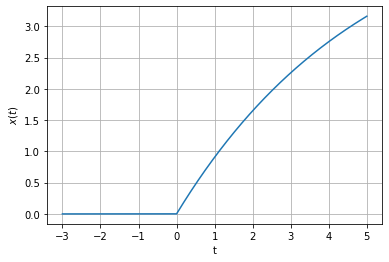
\includegraphics[width=\columnwidth] {Gate_Assignment_2_Fig_1.png}
    \caption{Step response $x(t)$ vs $t$}
    \label{Step response x(t)}
\end{figure}

\end{document}
